\chapter{Smooth steering}
\label{ch:smooth}

Every path so far is made of straight lines and arcs, joined end to end. Where
a line meets an arc, the curvature jumps from $0$ to $\pm\kmax$: the front
wheels would have to turn from straight to full lock in no time. A real
steering, turned by a motor or by a person, turns at a limited rate. This
chapter shows what that limit does to the paths, how to make the paths obey
it, and what it costs.

\section{The steering rate}

Let the steering turn at most at the rate $\omega$. The default is
$\omega = 40°$ per second, from straight to full lock in one second; it is
set by \code{max\_steer\_rate\_deg} in \code{mower.json}.

\begin{proposition}{Rate of change of the curvature}{sharpness}
  Driving at the speed $v$, a path whose curvature changes with the distance
  $s$ at most at the rate
  \[
    \Bigl|\frac{d\kappa}{ds}\Bigr| \le \sigma = \frac{\omega}{L\, v}
  \]
  asks the steering to turn at most at the rate $\omega$.
\end{proposition}

\begin{proof}
  With $\kappa = \tan\delta / L$ (Theorem~\ref{thm:bicycle}), $d\kappa/d\delta
  = 1/(L\cos^2\delta)$, and $ds = v\,dt$, so
  \[
    \frac{d\delta}{dt} = L \cos^2\!\delta \; v\, \frac{d\kappa}{ds},
    \qquad
    \Bigl|\frac{d\delta}{dt}\Bigr| \le L\, v\, \sigma = \omega,
  \]
  since $\cos^2\delta \le 1$.
\end{proof}

The bound is exact for a straight steering and cautious near full lock,
where the same change of steering changes the curvature more (by
$1/\cos^2 40° = 1.70$ times).

\begin{example}{From straight to full lock}{fullramp}
  In arcs the mower drives at $v = \SI{0.7}{\metre\per\second}$, so
  \[
    \sigma = \frac{0.698}{1.20 \times 0.7} = \SI{0.831}{\per\metre\squared},
    \qquad
    \ell_c = \frac{\kmax}{\sigma} = \frac{0.699}{0.831} = \SI{0.841}{\metre},
  \]
  where $\ell_c$ is the distance driven while the curvature grows from $0$
  to $\kmax$ (in \SI{1.20}{\second}). In reverse, at
  \SI{0.6}{\metre\per\second}, $\sigma = \SI{0.970}{\per\metre\squared}$.
\end{example}

\begin{definition}{Clothoid}{clothoid}
  A \emph{clothoid} (or Euler spiral) is a path whose curvature changes
  linearly with the distance: $\kappa(s) = \kappa_0 + \sigma s$. Its
  heading is $\theta(s) = \theta_0 + \kappa_0 s + \sigma s^2/2$ and its
  points are
  \[
    x(s) = x_0 + \int_0^s \cos\theta(u)\,du, \qquad
    y(s) = y_0 + \int_0^s \sin\theta(u)\,du,
  \]
  the Fresnel integrals, which have no closed form.
\end{definition}

The code represents a clothoid from $\kappa_0$ to $\kappa_1$ by twelve
short arcs, each with the curvature of the clothoid at its middle; the end
of the ramp of Example~\ref{ex:fullramp} is then within
\SI{0.3}{\milli\metre} of the exact one, and the path stays a list of
segments that the rest of the code already handles.

Where the mower stops to change direction, it can turn the steering while
standing: in the $t_{\mathrm{shift}} = \SI{2}{\second}$ of the stop, the
steering turns by up to $80°$, from full lock on one side to full lock on
the other. At a change of direction the curvature may still jump.

\section{A turn with ramps}

Replacing the jumps of curvature by ramps changes where a turn goes. The
simplest case is the U-turn at full lock.

\begin{proposition}{U-turn with ramps}{ccuturn}
  Let a ramp of length $\ell_c = \kmax/\sigma$ start at the origin with
  heading $0$ and end at $(x_c, y_c)$ with heading $\theta_c = \kmax
  \ell_c/2$. The path made of this ramp, an arc of radius $R = 1/\kmax$
  and the mirror image of the ramp turns the heading by $\pi$, ends at
  $(0, 2\Omega_y)$ and reaches $x = \Omega_x + R$, where
  \[
    \Omega = (\Omega_x, \Omega_y) = (x_c - R\sin\theta_c,\; y_c +
    R\cos\theta_c)
  \]
  is the centre of the arc. Its length is $2\ell_c + R(\pi - 2\theta_c)$.
\end{proposition}

\begin{proof}
  At the end of the ramp the curvature is $\kmax$, so the arc that follows
  has its centre at the distance $R$ to the left of the heading $\theta_c$:
  $\Omega = (x_c, y_c) + R(-\sin\theta_c, \cos\theta_c)$. The whole path is
  symmetric about the line $y = \Omega_y$ (the second ramp is the first
  driven backwards in the mirror), so it ends at the mirror image of the
  origin, $(0, 2\Omega_y)$, with the mirror heading $\pi$. The two ramps
  turn the heading by $\theta_c$ each, the arc by the rest, $\pi -
  2\theta_c$, on a length $R(\pi - 2\theta_c)$. The point of the arc
  furthest along $x$ is at $\Omega_x + R$.
\end{proof}

\begin{example}{The cost of the ramps}{ccnumbers}
  With $\ell_c = 0.841$ and $\sigma = 0.831$, numerical integration gives
  $x_c = 0.834$, $y_c = 0.082$ and $\theta_c = 0.294$ ($16.9°$), so
  \[
    \Omega = (0.834 - 1.430 \sin 0.294,\; 0.082 + 1.430 \cos 0.294) =
    (0.419,\; 1.451).
  \]
  The U-turn is $2\Omega_y = \SI{2.90}{\metre}$ wide instead of $2R =
  \SI{2.86}{\metre}$, it goes \SI{0.42}{\metre} further, and it is
  $2 \times 0.841 + 1.430\,(\pi - 0.588) = \SI{5.33}{\metre}$ long instead
  of $\pi R = \SI{4.49}{\metre}$: \SI{1.2}{\second} more at
  \SI{0.7}{\metre\per\second}.
\end{example}

Fraichard and Scheuer~\cite{fraichard2004reeds} build on this observation
the continuous-curvature analogues of the Reeds--Shepp paths, with the
circles of radius $R$ replaced by circles of radius $|\Omega|$; Sabelhaus
and others~\cite{sabelhaus2013using} use continuous-curvature paths for the
headland turns of agricultural machines. The code here takes a more direct
route.

\section{Smoothing a path}

The code makes any path of the earlier chapters obey the steering rate,
while keeping it anchored where it matters.

\begin{description}
  \item[Anchors.]
    \leavevmode\\
    The middle of every straight segment at least \SI{1.5}{\metre} long
    (most of all, the passes) is an \emph{anchor}: there the curvature is
    zero, and the pose must stay where it is. The path is cut at the
    anchors into \emph{runs}.
  \item[Ramps.]
    \leavevmode\\
    In a run, every change of curvature while moving becomes a ramp of slope
    $\sigma$ (for the speed of the segment after it); the ramps take
    distance and turn the heading, so the run no longer ends at its anchor.
  \item[Adjustment.]
    \leavevmode\\
    The lengths of the segments of the run and the curvatures of its arcs
    (at most $\kmax$ in size) are adjusted until the run ends again at the
    anchor: three equations (the end pose), solved by Levenberg--Marquardt,
    a Gauss--Newton method that shortens its steps when they do not
    reduce the error.
  \item[Continuation.]
    \leavevmode\\
    Started directly from the original lengths, the adjustment can get
    stuck. The ramps are therefore grown in five stages, from a fifth of
    their length to the full length, each stage starting from the solution
    of the previous one: at length zero the original run is the solution,
    and each stage is a small change.
  \item[Other words.]
    \leavevmode\\
    If the adjustment fails, or the smoothed run leaves the lawn, the other
    Reeds--Shepp words between the same poses are tried, fastest first.
\end{description}

Figure~\ref{fig:clothoid} shows two turns before and after. A ramp-shaped
turn always takes longer than the original: a ramp covers the same angle
as half its length at full lock, so the turn needs a longer arc of
curvature below $\kmax$, and the speed in it is the speed of arcs.

\begin{figure}[ht]
  \centering
  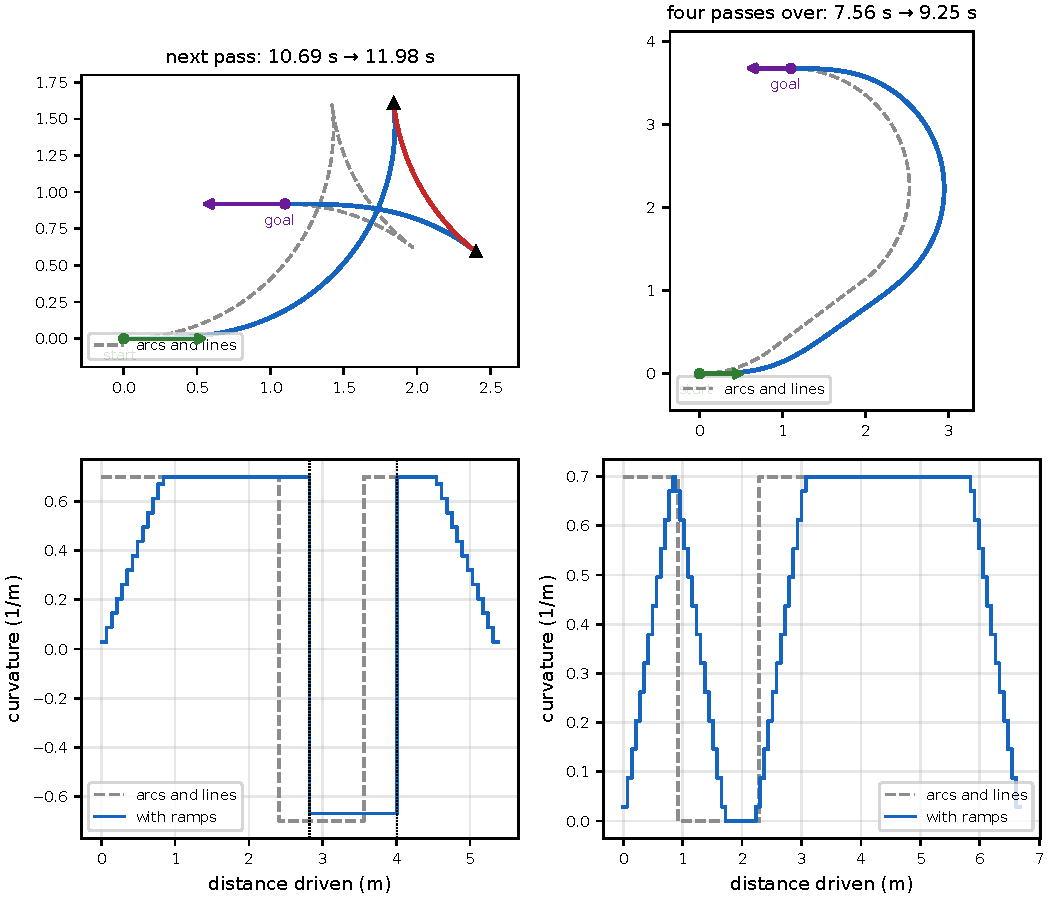
\includegraphics[width=\textwidth]{figures/clothoid}
  \caption{Turns from the end of a pass (green) to the next pass driven the
    other way (purple), as arcs and lines (dashed grey) and with ramps (blue
    forward, red reverse). Bottom: the curvature along each path; the
    vertical dotted lines are the changes of direction, where the steering
    turns during the stop. Left: the three-point turn into the next pass.
    Right: the forward turn four passes over, whose first arc no longer
    reaches full lock.}
  \label{fig:clothoid}
\end{figure}

\section{Planning with smooth turns}

Smoothing a plan after the fact is not enough: the turns with ramps need
more room (Example~\ref{ex:ccnumbers}), and the order of the passes was
chosen with the times of the turns without ramps. With the option
\code{smooth}, the planner uses turns with ramps everywhere a turn is
chosen: in the times $T(j)$ of the order of the passes
(Chapter~\ref{ch:swaths}), in the room $a_{\mathrm{turn}}$ that sets the
number of headland passes (Proposition~\ref{prop:headlandcount}), and in
the turns between passes; the rest of the path (the headland, the
transfers) is smoothed at the end.

\begin{figure}[ht]
  \centering
  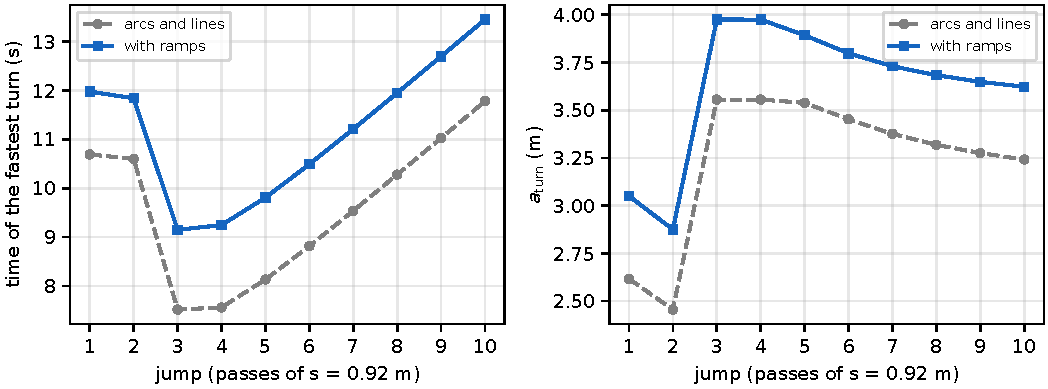
\includegraphics[width=\textwidth]{figures/smooth_turns}
  \caption{The turns of Figure~\ref{fig:turntimes} with ramps (blue) and
    without (dashed grey). Left: the time of the fastest turn, about
    \SI{1.3}{\second} longer for the three-point turns and
    \SI{1.6}{\second} for the forward ones. Right: the room beyond the rear
    axle, \SI{0.4}{\metre} more.}
  \label{fig:smoothturns}
\end{figure}

The turns with ramps need more room: $a_{\mathrm{turn}} = \SI{3.05}{\metre}$
for the three-point turn and \SI{3.98}{\metre} for the forward turns, so by
Proposition~\ref{prop:headlandcount}
\[
  n = 1 + \Bigl\lceil \frac{3.051 + 0.05 - 1.90}{0.92} \Bigr\rceil = 3
  \quad\text{and}\quad
  n = 1 + \Bigl\lceil \frac{3.975 + 0.05 - 1.90}{0.92} \Bigr\rceil = 4
\]
headland passes (with $d + r + c_1 + w/2 = 0.80 + 0.615 + 0.485 =
\SI{1.90}{\metre}$), one more than without ramps in both cases.
Figure~\ref{fig:smoothplans} and the table below show the complete plans.

\begin{figure}[p]
  \centering
  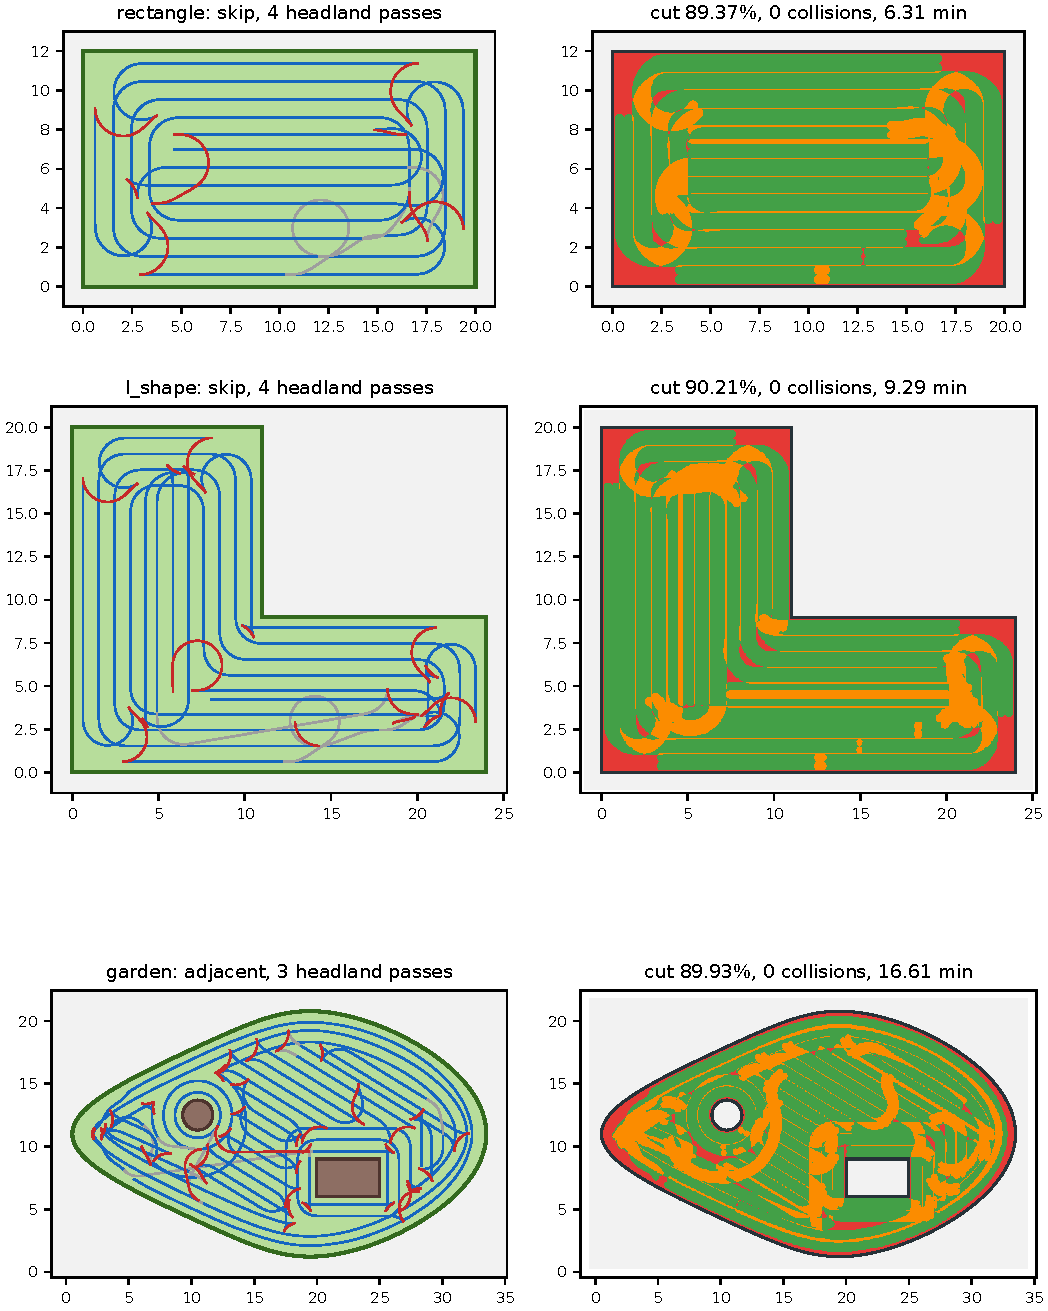
\includegraphics[width=\textwidth]{figures/smooth_plans}
  \caption{The complete planner with turns and paths that the steering can
    follow (curvature ramps everywhere), on the three example lawns. Left:
    the path of the rear axle (blue forward, red reverse, grey blades off).
    Right: the grass cut (green once, orange twice, red missed).}
  \label{fig:smoothplans}
\end{figure}

\begin{center}
\begin{tabular}{@{}lrrrrr@{}}
  \toprule
  & \multicolumn{2}{c}{arcs and lines} & \multicolumn{3}{c}{with ramps} \\
  lawn & cut & time & cut & time & jumps left \\
  \midrule
  rectangle & 91.9\% & \SI{5.71}{\minute} & 89.4\% & \SI{6.31}{\minute} & 0 \\
  L-shape & 92.3\% & \SI{8.40}{\minute} & 90.2\% & \SI{9.29}{\minute} & 0 \\
  garden & 90.6\% & \SI{15.78}{\minute} & 89.9\% & \SI{16.61}{\minute} & 211 \\
  \bottomrule
\end{tabular}
\end{center}

The ramps cost about \SI{10}{\percent} of the time on the rectangle and the
L-shape, and two points of coverage: the extra headland pass has corners of
its own, and the turns with ramps leave slightly larger gaps where they
meet the headland. On the garden they cost \SI{5}{\percent}: much of its
time was already spent on the arcs of its curved border, at the speed of
arcs. The last column counts the places where the curvature still changes
faster than the steering can follow (by more than $\sigma$ times
\SI{15}{\centi\metre}). On the rectangle and the L-shape there are none. On
the garden, 211 remain, in seven stretches of its curved headland made of
many short arcs, where the smoothed path either drifted or pushed the mower
into the margin, and which were kept as planned; there the steering lags
behind the plan, and the next chapter measures what that costs.

\begin{inwords}
  A steering that turns at a limited speed cannot follow the sudden changes
  of curvature of arcs and lines. Replacing each change by a ramp, a
  clothoid, makes every turn a little wider, longer and slower. Planning
  with these turns from the start keeps the mower on the lawn; the price
  is paid in the turns, about a second and a half each.
\end{inwords}

\begin{incode}
  \code{mowersim/smooth.py}: \code{sharpness}
  (Proposition~\ref{prop:sharpness}), \code{ramp} (Definition~\ref{def:clothoid}),
  \code{build}, \code{smooth\_run} (adjustment and continuation),
  \code{smooth} (a whole trajectory), \code{curvature\_jumps}.
  \code{connect(..., smooth=True)} in \code{mowersim/planning/common.py},
  \code{fastest\_turn}, \code{turn\_time} and \code{turn\_ahead} with
  \code{smooth=True}, and \code{plan(..., smooth=True)}. From the command
  line:
  \begin{verbatim}
python -m mowersim plan lawns/garden.json --smooth
  \end{verbatim}
\end{incode}
